\section{Introduction}

\subsubsection{Importance of analysing watch time.} YouTube starts to stress on watch time rather than view number.

\subsubsection{A metric to quantify video quality.} Quality of video is a loose defined concept. We use video watch percentage as a proxy to measure video quality.

\subsubsection{Cold-start predicting watch percentage}

%----------------------------------------------------------------------------------------

\section{Related work}

\subsubsection{YouTube watching behavior} Video watch time associates with popularity metrics (e.g., view count, the number of comments and shares) and user reaction (e.g., sentiment polarity of comments, the number of likes and dislikes) collectively \cite{park:2016engagement}. However, their observations base on a prior observation period, while our focus is different, without observing an early reaction from video audiences, can we predict watch percentage from a cold start setting up? Or can we classify a bunch of quality videos?

\subsubsection{Model of predicting future view count} Peeking strategy and \textit{ex-ante} prediction \cite{martin:2016exploring}.

%----------------------------------------------------------------------------------------

\section{Data and measurement}

In order to study YouTube watching behavior, we built a tool to collect user watching statistics on a daily basis. In this section, we first introduce a large dataset that contains rich features from nearly 20 million YouTube videos, then provide intuitive measurements.

\subsection{Data Collection}

\noindent\textbf{Random Videos:} To obtain a sample of YouTube videos, we used Twitter appearance as a selecting policy. With the help of Twitter Streaming API, first we crawled 202 million tweets that contained "YouTube" keyword over two months period, from July 1st, 2016 to August 30th, 2016. We then parsed the associated shortened URL and only considered tweets that linked to a genuine YouTube video page. Out of these, 36 million video IDs were identified. Finally, we used YouTube Data API and YTCrawl tool \cite{yu:2015lifecyle} to acquire video metadata and daily viewing statistics respectively. After accounting the effects of Twitter sampling, video attrition and private statistics, our Random Videos resulted in a total set of nearly 20 million YouTube videos. Furthermore, we grouped these random videos by category to constitute Random Music dataset, Random News dataset, et cetera. We regarded Random Videos as an approximation of overall YouTube videos.

The most two prominent and valuable statistics of this dataset are daily watch time \textit{WatchT} and daily view count \textit{View}. Upon those, we can derive portion of watching \textit{WatchP} that an average user spends per view at a daily granularity by performing a pairwise division \textit{WatchT}/\textit{View}/duration. We user this series data \textit{WatchP} to reveal watching behavior temporal trend (see section xx). Besides, we extract \textit{WatchP@180} as \textit{WatchT@180}/\textit{View@180}/duration to approximate the intrinsic property.

\noindent\textbf{Quality Videos:} The Quality Videos dataset consists of two parts, VEVO dataset and Top News dataset. VEVO dataset contains videos from all verified VEVO accounts on YouTube platform; Top News dataset features top 100 most viewed News channels, as reported by external source \footnote{https://vidstatsx.com/youtube-top-100-most-viewed-news-politics}. The number of videos and corresponding statistics in each dataset can be found in Table~\ref{table:1}.

\begin{table*}
  \caption{Overview of datasets}
  \label{table:1}
  \begin{tabular}{ccccc}
    \toprule
    Dataset & \#Videos & \#Channels & \#Avg Views & \#Avg Watch Time/View \\
    \midrule
    Random Videos & 19,464,997 &  & \\ 
    Random Music & 2,179,330 & 649,895 & \\ 
    VEVO & 72,488 & 14,342 & \\
    Random News & 1,079,149 & 105,853 & \\
    Top News & 29,732 & 91 & \\
  \bottomrule
\end{tabular}
\end{table*}

\subsection{Watch percentage temporal pattern}

For most videos, watch percentage behaves like a linear trend, most time flat. (How to present this story?)

Can we summary a few types of temporal pattern? (R.Crane and D.Sornette, viral videos short paper)

Output: a bunch of different temporal patterns, explained by videos plot.


\subsection{Proxy of Video Quality}
Since watch percentage doesn't vary much, can we use watch percentage as a proxy of video quality, taking duration and category (maybe age?) as control variable.

Thus we use external resource to validate video quality. Video quality is a loose defined concept. It's a mix of production quality, content topic and channel profile. [refer to Figure 1 or so, high quality videos appear on the top left.]

\begin{figure}
    \centering
    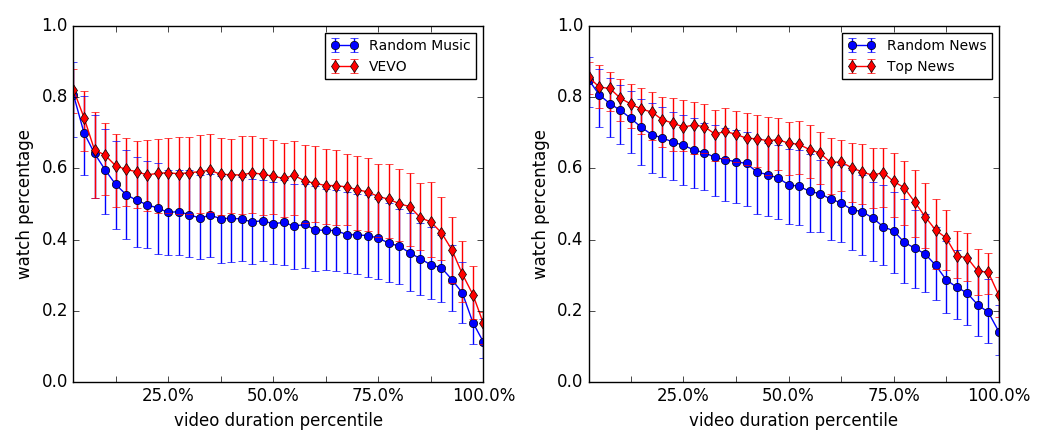
\includegraphics[scale=0.32]{image/external_source_comp.png}
    \caption{External Source Validation}
\end{figure}

Output: quality video dataset sit on top of random video dataset.


\subsection{Old videos and dedicated audience}

Hypotheses: when a video gets older, it will attract more dedicated audience thus appears as a growing watch percentage, even though views decrease.

Questions here: how to define old? (moving truncated?) and how to express growth?

Note: fewer views inevitable result in larger variance of watch percentage.

Output: whether or not it hits dedicated audience?


%----------------------------------------------------------------------------------------

\section{Cold start watch behavior prediction}

\subsection{Classify Quality Videos}
How well can this model with a floating quality threshold?

input: a new video, with metadata only (video features, user vector)

output: is this a quality video? (appear above the top x\% of duration percentile plot)

method: classification task; category, duration as control variable.

setup: 

\subsection{Predict Watch Percentage}
input: a new video, with metadata only (video features, user vector)

output: what's the watch percentage by day 30? performance matrix to select features

method: regression task; category, duration as control variable.

setup: 

%----------------------------------------------------------------------------------------

\section{Integrate with HIP: Predict future watch time}
HIP model, learn a set of parameters to map dailyshare to dailywatch

Question: does this model work better with watch percentage plugged in?

input: a new video, with observed dailyshare, dailywatch, daily watch percentage

output: a line that fit video watch time in entire (120? 30?) lifecycle, explain the video quality.

method: HIP and modified HIP
%\end{document}  % This is where a 'short' article might terminate



%\appendix
%%Appendix A
%\section{Headings in Appendices}
%The rules about hierarchical headings discussed above for
%the body of the article are different in the appendices.
%In the \textbf{appendix} environment, the command
%\textbf{section} is used to
%indicate the start of each Appendix, with alphabetic order
%designation (i.e., the first is A, the second B, etc.) and
%a title (if you include one).  So, if you need
%hierarchical structure
%\textit{within} an Appendix, start with \textbf{subsection} as the
%highest level. Here is an outline of the body of this
%document in Appendix-appropriate form:
%\subsection{Introduction}
%\subsection{The Body of the Paper}
%\subsubsection{Type Changes and  Special Characters}
%\subsubsection{Math Equations}
%\paragraph{Inline (In-text) Equations}
%\paragraph{Display Equations}
%\subsubsection{Citations}
%\subsubsection{Tables}
%\subsubsection{Figures}
%\subsubsection{Theorem-like Constructs}
%\subsubsection*{A Caveat for the \TeX\ Expert}
%\subsection{Conclusions}
%\subsection{References}
%Generated by bibtex from your \texttt{.bib} file.  Run latex,
%then bibtex, then latex twice (to resolve references)
%to create the \texttt{.bbl} file.  Insert that \texttt{.bbl}
%file into the \texttt{.tex} source file and comment out
%the command \texttt{{\char'134}thebibliography}.
%% This next section command marks the start of
%% Appendix B, and does not continue the present hierarchy
%\section{More Help for the Hardy}
%
%Of course, reading the source code is always useful.  The file
%\path{acmart.pdf} contains both the user guide and the commented
%code.
%
%\begin{acks}
%  The authors would like to thank Dr. Yuhua Li for providing the
%  matlab code of  the \textit{BEPS} method. 
%
%  The authors would also like to thank the anonymous referees for
%  their valuable comments and helpful suggestions. The work is
%  supported by the \grantsponsor{GS501100001809}{National Natural
%    Science Foundation of
%    China}{http://dx.doi.org/10.13039/501100001809} under Grant
%  No.:~\grantnum{GS501100001809}{61273304}
%  and~\grantnum[http://www.nnsf.cn/youngscientsts]{GS501100001809}{Young
%    Scientsts' Support Program}.
%
%\end{acks}
